\documentclass[12pt, a4paper]{article}

\usepackage{graphicx}
\usepackage{float}
\usepackage{hyperref}
\usepackage{siunitx}

\begin{document}
	\pagenumbering{gobble}
		\begin{titlepage}
			\centering
			{\LARGE Electronics Practical 4 \par}
			\vspace*{1.5cm}
			{\large Q. Kruger, 216008466 \par}
			{\large R. de Bruyn, 216054484 \par}
			{\large W. B. Richardson, 201578882 \par}
			\vspace*{1.2cm}
			{\large \today}
			\vspace*{\fill}
			% 
\includegraphics[width=\textwidth]{img/UJ.jpg}
			\vspace*{\fill}
		\end{titlepage}
		\tableofcontents
		\listoffigures
		\newpage
		\pagenumbering{arabic}
	\section{Theoretical Background} % (fold)
	\label{sub:theoretical_background}
	To design an amplifier circuit we require a number of parameters:
	\begin{enumerate}
	 	\item The collector resistor $R_C$
	 	\item The emitter resistor $R_E$
	 	\item The base current $I_B$
	 	\item The base voltage $V_{BB}$
	 	\item The base resistor $R_B$
	 	\item A number of capacitors
	\end{enumerate}

	These parametes influence the Q-point of the transistor (the optimal point at which maximum amplification results). The Q-point is transistor specific and the values of the unknown capacitances and resitances.

	Consider the circuit as shown by Figure \ref{fig:amplifier_circuit} for reference to the discussion of the steps to follow in finding the required resistance and capacitance values to implement an amplifier.

	%Include the image that the explanation is about from an LTSpice implementation of instructables
	\begin{figure}[H]
		\centering
		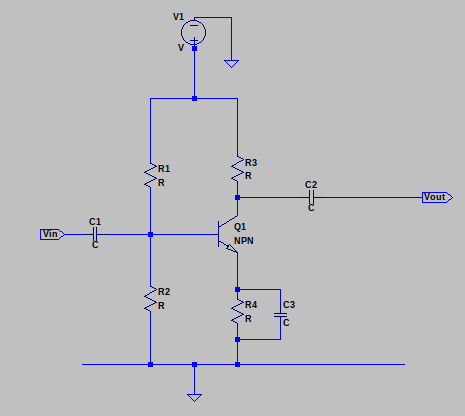
\includegraphics[width=0.7\textwidth]{Images/amplifier_circuit.png}
		\caption{Amplifier circuit}
		\label{fig:amplifier_circuit}
	\end{figure}

	A transistor operates as an amplifier in the forward active region. To operate the transistor as an amplifier we require the Q-point to be in the center of the DC load line. In order for the Q-point to be the center point of the load line the following steps need to be employed to find appropriate values of the resistances and capacitances. The steps are as follows:\\

	\textit{(Throughout the discussion of the steps to follow, we assume a supply voltage $V_1$ as $15V$ and a frequency of $95MHz$)}.
	\begin{enumerate}
		\item Finding $R_3$ - collector resistor\\
		The collector voltage should be half that of the supply voltage, this allows equal execution of the signal up and down. Using ohms law, the resulting resistor can be obtained 
		\item Finding $R_4$ - emitter resistor\\
		For an acceptable level of DC stability, we require that the emitter voltage be $10\%$ of the supply voltage. Again, using ohms law and the approximation that the emitter current is that of the collector current we can find the emitter resistor value.
		\item Finding base current $I_B$\\
		From the relationship of transistor currents given as $I_C = I_B \times \beta$, the required base current can be calculated, given as $I_B = \frac{I_C}{\beta}$
		\item Finding base voltage $V_{BB}$\\
		Base voltage $V_{BB}$ is given as the sum of the forward-biased base-emitter voltage (for Si, this value is $0.6V$ and for Ge, this value is $0.2V$), and the base voltage (this result comes from Kirchoff's voltage law).
		\item Finding the base resistance - values of resistors $R_1$ and $R_2$\\
		The base resistance is given as the ration of t he 2 resistors $R_1$ and $R_2$. Using voltage divider rule to get the required base voltage as was calculated in the previous step. The voltage divider rule is given as $V_{BB} = \frac{R_2}{R_1 + R_2}$.
		\\\textit{The required base voltage can be approximated so that resistor values that are readily available can be used.} 
		\item Emitter bypass capacitor - $C_3$
		Without the capacitor, the gain of the input AC signal is merely given as $\frac{R_3}{R_4}$. To increase this gain, a capacitor needs to be placed in parallel with the emitter resistor $R_4$ with an impedance value equal to that of the resistor $R_4$ at the frequency of the input AC signal. Thus the equation giving us this result is $C = \frac{1}{2\pi\times f \times X_C}$ where $X_C = R_4$. 
		\item Find the input capacitor value - $C_1$\\
		The impedance of this capacitor must be that of the input impedance at the input frequency to give it a $-3dB$ fall at this frequency. The formula for calculating the input capacitance is given as $C = \frac{1}{2\pi\times R \times f}$
		\item Find the output capacitor value - $C_2$\\
		The capacitor impedance is chosen to equal the circuit impedance. The circuit impedance is taken to be the sum of the emitter follower output resistance plus the resistance of the load. Again the equation to be used is given as $C = \frac{1}{2\pi \times R \times f}$.

	\end{enumerate}


	
	% subsection theoretical_background (end)

	\section{Experimental Method} % (fold)
	\label{sub:experimental_method}
	The student number used to implement this circuit was 216054484. The relevant parameters are shown below:
	\begin{enumerate}
		\item Voltage gain - 6.5
		\item Source output resistance - $2.2$K 
		\item Lower corner frequency - $90$ Hz
		\item Upper corner frequency - $28$ KHz
	\end{enumerate}
	Other component values were calculated as explained in the theoretical background section of this report. The component values are shown in Figure \ref{fig:lab_circuit}

	\begin{figure}[H]
		\centering
		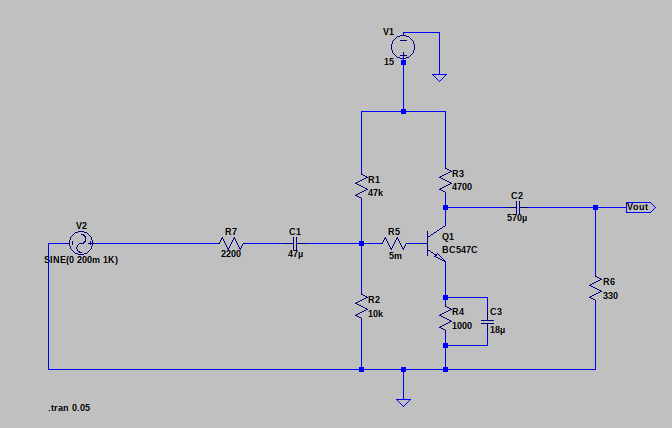
\includegraphics[width=0.7\textwidth]{Images/lab_circuit.png}
		\caption{Circuit as set up for this experiment}
		\label{fig:lab_circuit}
	\end{figure}
	
	A list of the components that resulted from our design are given below:
	\begin{enumerate}
		\item BC547C Transistor
		\item 47K Resistor
		\item 10K Resistor
		\item 4.7K Resistor
		\item 1K Resistor
		\item 2.2K Resistor
		\item 10 $\mu$F Capacitor
		\item 570 $\mu$F Capacitor
		\item 47 $\mu$F Capacitor
	\end{enumerate}
	% subsection experimental_method (end)

	\section{Results} % (fold)
	\label{sub:results} 
	By running the simulation in LTspice with a sinusoidal input with a peak value of $200$mV and a collector supply of 15V DC, the following results were obtained as shown in the figures respectively for the input and the output (Figure \ref{fig:input_signal} and Figure \ref{fig:output_signal})

	\begin{figure}[H]
		\centering
		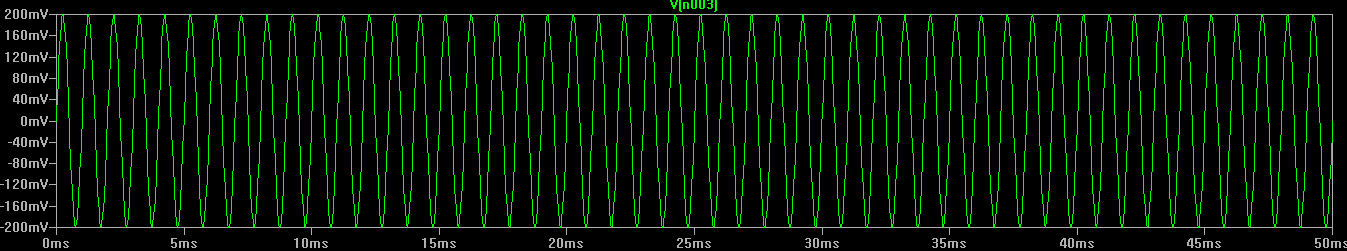
\includegraphics[width=0.7\textwidth]{Images/input_signal.png}
		\caption{Input signal to the amplifier circuit}
		\label{fig:input_signal}
	\end{figure}
	
	\begin{figure}[H]
		\centering
		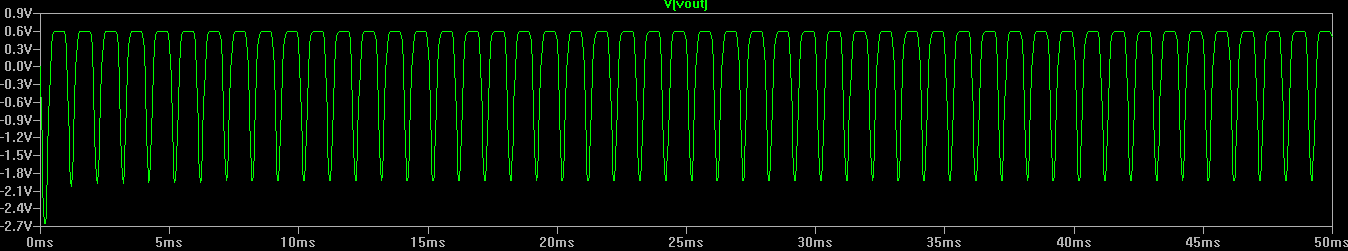
\includegraphics[width=0.7\textwidth]{Images/output_signal.png}
		\caption{Output signal to the amplifier circuit}
		\label{fig:output_signal}
	\end{figure}


	% subsection results (end)

	\section{Conclusions} % (fold)
	The gain at the output was given as 2.7V measure from peak to peak. This correlates with the desired circuit behavior of increasing the voltage at the input with a gain of 6.75. This is close to the design goal, we were not able to get the exact gain due to being limited to the e12 series resistors.
	\label{sub:conclusions}

	
	% subsection conclusions (end)
\end{document}